\chapter[Identificación de métodos builders]{Enfoques para la identificación de Métodos Builders}
\label{cap:builders}
\pp{Reemplazar builders por generadores de objetos o algo parecido}

% 



% 1- Definir builders
% Falta definir lo que son builders
En el contexto del desarrollo de software, los métodos generadores de objetos (también conocidos como métodos \emph{builders} de una API) son aquellos métodos específicos diseñados para crear, modificar y retornar objetos de una clase en particular. Este subconjunto de métodos es capaz de generar cualquier configuración posible de la API. La identificación manual de estos métodos requiere un análisis exhaustivo de la lógica y el código de la API.
% 2- Por qué es importante
Los métodos \emph{builders} son especialmente útiles cuando se necesita crear objetos que requieren una serie de pasos o configuraciones específicas. En muchas aplicaciones, especialmente en sistemas de software grandes y complejos, los objetos pueden tener múltiples atributos y configuraciones que deben especificarse para su creación. Los métodos generadores de objetos simplifican este proceso al proporcionar métodos concisos para crear diferentes tipos de objetos de una API.

\cacho{quiero decir que para recrear configuraciones de la API, es complejo utilizar los metodos de la API}
Esta funcionalidad es especialmente relevante en las pruebas unitarias, ya que permite crear objetos con configuraciones específicas para probar diferentes escenarios y casos de uso. Estas configuraciones solo se crean mediante combinaciones de llamadas a los métodos generadores de objetos.

Es importante destacar que estas configuraciones deben estar limitadas para poder crearlas de manera eficiente y efectiva. Para lograr esto, se introduce el concepto de "scope", que representa el límite en el número de objetos y rangos para los tipos de datos, como se describe en \cite{jackson2006, frias2005dynalloy}.
\cacho{Chequear la cita, lo saque del paper de Efficient Bounded Model Checking of Heap-Manipulating Programs using Tight Field Bounds}. La justificación para utilizar conjuntos acotados de objetos es similar a la hipótesis de alcance de la cota pequeña \cite{Andoni:2003}. Si un conjunto de métodos no puede utilizarse para construir objetos pequeños que permitan diferenciarlo de otro conjunto de métodos, es poco probable que estos dos conjuntos puedan distinguirse con objetos más grandes.

\cacho{No se como enganchar y explicar lo de scope para que quede claro la deficinion. Chequear esto.}

% Esto puede tener gran importancia en las pruebas unitarias, ya que permiten crear objetos con configuraciones específicas para probar diferentes escenarios y casos de uso. Estas configuraciones solo se crean con la combinaciones de llamadas a los métodos generadores de objetos. 
% Es importante remarcar que estas configuraciones deben estar limitadas para poder crearlas de manera efictivas y eficientes. Para esto se intruduce la idea de \emph{scope} que es el limite de numeros de objectos y rangos para los tipos de datos tal como se describe en \cite{jackson2006, frias2005dynalloy}
%  La justificación para utilizar conjuntos acotados de objetos es similar a la hipótesis de alcance de la cota pequeña \cite{Andoni:2003}. Si un conjunto de métodos no puede utilizarse para construir objetos pequeños que permitan diferenciarlo de otro conjunto de métodos, es poco probable que estos dos conjuntos puedan distinguirse con objetos más grandes. 


En el contexto de una API, el conjunto de métodos generadores de objetos debe ser suficiente y minimal para garantizar un manejo eficiente y completo de las configuraciones de objetos posibles.

La propiedad de ``suficiente'' implica que este conjunto de métodos debe ofrecer todas las opciones y parámetros necesarios para configurar completamente un objeto de la API. En otras palabras, con estos métodos, los usuarios deben poder generar cualquier configuración deseada de objetos dentro de la API. Esta característica es fundamental, ya que garantiza que el subconjunto de métodos generadores sea competente y abarque todas las posibilidades que la API puede ofrecer.

Por otro lado, la propiedad de ``minimal'' es igualmente importante que la propiedad de suficiencia. Al referirnos a que los métodos deben ser minimalistas, nos referimos a que deben ser los más simples \cacho{No se si es la palabra acorde} y el conjunto debe tener la menor cantidad posible de métodos. Esto quiere decir, que cada método debe cumplir una función específica y claramente definida, sin redundancia innecesaria. La ausencia de cualquier método de este conjunto podría significar que exista al menos una configuración de la API que no se pueda recrear o generar. Especialmente en situaciones donde los objetos pueden tener múltiples atributos o propiedades, la falta de la propiedad de minimalismo del subconjunto de métodos puede generar una explosión de combinaciones de los mismos, dificultando el proceso de generación.

% Suficiente (indep. de los algoritmos)


% Minimos (indep. de los algoritmos)



\begin{table}[H]
\center
{\scriptsize
\begin{tabular}{|l|l|l|l|}
\hline
No. &Tipo de retorno & Nombre del Método & Observador? \\
\hline
    0 && NCL() & no \\
    1& & NCL(int) & no \\
    2&& NCL(Collection) & no \\
    3&boolean & add(Object) & no \\
    4&void&add(int,Object) & no \\
    5&boolean&addAll(Collection) & no\\
    6&boolean&addAll(int,Collection) & no \\
    7&boolean&addFirst(Object) & no \\
    8&boolean&addLast(Object) & no\\
    9&void&clear() & no\\
    10&boolean&contains(Object) & si \\
    11&boolean&containsAll(Collection) & si \\
    12&boolean&equals(Object) & si \\
    13&Object&get(int) & si\\
    14&Object&getFirst() & si \\
    15&Object&getLast() & si\\
    16&int&indexOf(Object) & si\\
    17&boolean&isEmpty() & si\\
    18&Iterator&iterator() & no\\
    19&int&lastIndexOf(Object) & si \\
    20&ListIterator&listIterator() &no \\
    21&ListIterator&listIterator(int) & no\\
    22&Object&remove(int) &no\\
    23&boolean&remove(Object) & no \\
    24&boolean&removeAll(Collection) & no \\
    25&Object&removeFirst() &no\\
    26&Object&removeLast() &no\\
    27&boolean&retainAll(Collection) &no \\
    28&Object&set(int,Object) &no\\
    29&int&size() &si \\
    30&List&subList(int,int) & no \\
    31&Object[]&toArray() & si \\
    32&Object[]&toArray(Object[]) &si\\
    33&String&toString() & si \\
\hline
\end{tabular}
}
\caption{Apache's NodeCachingLinkedList API}
\label{tab:ncl-api}
\end{table} 

Vamos a motivar estas definiciones mediante un ejemplo de una API. La estructura de datos NodeCachingLinkedList (NCL) de Apache \cite{apache} consta de una lista principal circular doblemente enlazada que contiene los elementos de la colección y una lista secundaria simplemente enlazada que actúa como caché para los nodos que se han `eliminado de la lista principal. Los nodos almacenados en la caché pueden ser reutilizados y añadidos de nuevo a la lista principal al insertar elementos en ella. Gracias a su caché, en las aplicaciones en las que las inserciones y eliminaciones de la lista son muy frecuentes, NCL puede reducir significativamente la sobrecarga necesaria para la asignación de memoria y la recolección de basura de los nodos. 
Como ilustración, la Figura~\ref{fig:ncl-instances} muestra las tres instancias de NCL que se pueden construir con exactamente dos nodos (scope).
\cacho{Chequear definir antes SCOPE}

\begin{figure}[H]
    \centering
    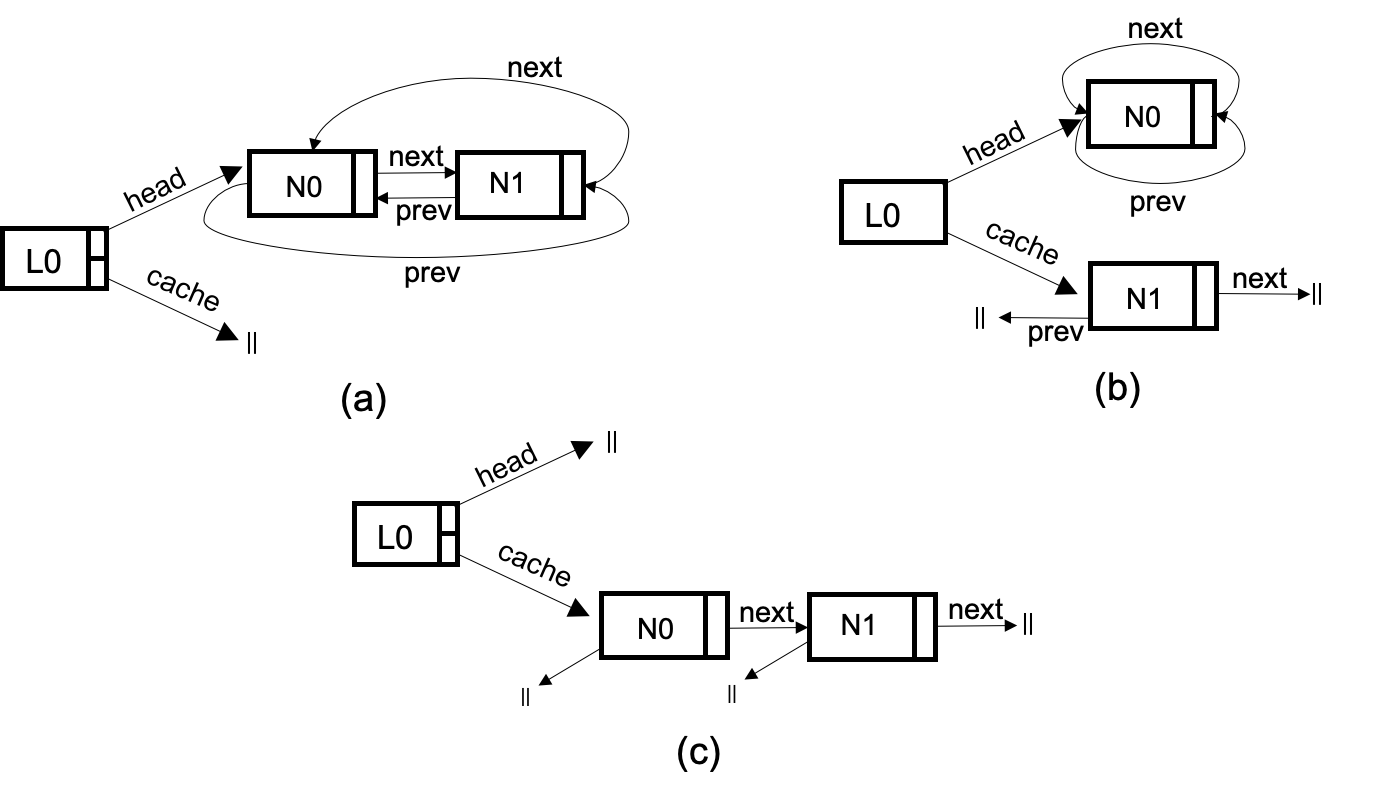
\includegraphics[width=0.85\textwidth]{NCL-instances.png}
    \caption{Tres instancias de NodeCachingLinkedList con exactamente dos nodos}
    \label{fig:ncl-instances}
\end{figure}


NCL tiene una API muy completa, como se muestra en la Tabla~\ref{tab:ncl-api}.
Sin embargo, para construir cualquier objeto de NCL hasta un \emph{scope} dado, solo se necesitan algunos métodos de la API. Por ejemplo, las combinaciones de los métodos en la Figura~\ref{fig:NCLbuilders}, cuando se instancian con los parámetros
apropiados, se pueden utilizar para construir cualquier objeto de NCL.
Por lo tanto, los métodos de la figura \ref{fig:NCLbuilders} son un ejemplo de un conjunto suficiente de métodos generadores de objetos para NCL
\\
\begin{lstlisting}[numbers=none,label=fig:NCLbuilders, caption=Conjunto de metodos sufiente para NCL]
  (0)  NodeCachingLinkedList()
  (7)  addFirst(Object)
  (25) removeFirst()
\end{lstlisting}

 Hay que tener en cuenta que, después de utilizar el método constructor de las clases NCL, la lista principal de NCL se puede completar simplemente utilizando el método \texttt{addFirst}. Sin embargo, si queremos generar instancias en las que la lista caché no esté vacía, podemos hacerlo a través del método \texttt{removeFirst}, como sugiere el conjunto suficiente de métodos generadores. Además, los métodos generadores de la figura~\ref{fig:NCLbuilders} también son mínimos, ya que la falta de alguno de ellos implicaría que algunos objetos de NCL ya no se pueden construir bajo el scope deseado.

Hay que tener en cuenta que puede haber muchos conjuntos de genereadores suficientes. Por ejemplo, se pueden obtener métodos generadores suficientes reemplazando el método \texttt{addFirst} en la Figura~\ref{fig:NCLbuilders} por cualquier otra variante de \texttt{add} que se muestra en la Figura~\ref{fig:NCLadds}, ya que para cualquier manera de llenar la lista principal de NCL con \texttt{addFirst}, existe una forma diferente de construir el mismo objeto utilizando otra variante de \texttt{add} (quizás invocada con diferentes parámetros y cambiando el orden de ejecución).
\\
\begin{lstlisting}[numbers=none,label=fig:NCLadds, caption=Variantes del método 'Add' que puedo ser utilizado para rellanar la lista principal en NCL, captionpos=b, frame=tb , basicstyle=\scriptsize]
  (3) add(Object)
  (4) add(int,Object)
  (7) addFirst(Object)
  (8) addLast(Object)
\end{lstlisting}

% Además, es importante remarcar la importancia de obtener subconjuntos que sean mínimos\pp{acá aparece recién la definición de minímos}, lo que significa que 
% no contengan métodos adicionales. Esto es crucial para
% utilizar la combinación de estos métodos en la construcción de objetos. Cuantos
% más métodos tenga el subconjunto de builders, más costosa será la combinación de
% los mismos para generar los objetos 
% \pp{no está definido como se piensa generar
% los objetos}.

Como explicamos al principio, existen dos propiedades que deseamos que tengan los subconjuntos de métodos generadores de objetos. Primero deseamos obtener subconjuntos de métodos que sean suficientes, por ejemplo, los siguientes conjuntos son suficientes de NCL:
\\
\cacho{HAgo referencia al listing o lo dejo en linea como esta?}

\begin{lstlisting}[numbers=none,label=fig:NCLnoMin, frame=tb , basicstyle=\scriptsize]
  (0)  NodeCachingLinkedList()
  (7)  addFirst(Object)
  (3)  addF(Object)
  (25) removeFirst()
\end{lstlisting}

\begin{lstlisting}[numbers=none,label=fig:NCLnoMin1, caption= Conjuntos de metodos builders suficientes pero no mínimos, captionpos=b, frame=tb , basicstyle=\scriptsize]
  (0)  NodeCachingLinkedList()
  (7)  addFirst(Object)
  (3)  remove(Object)
  (25) removeFirst()
\end{lstlisting}

También observamos que cuanto más simples sean los parámetros de una rutina, más
fácil será utilizarla para generar entradas en el contexto de un análisis de
programas. Por ejemplo, entre las alternativas de rutinas para insertar datos en
la lista principal de NCL (Figura.~\ref{fig:NCLadds}), \texttt{add(int,Object)}
recibe más parámetros que los otros tres métodos, por lo tanto es más difícil generar parámetros para brindale a esta rutina a la hora de generar entradas \pp{No está definido como se generarían entradas}. Esto hace que las otras tres alternativas tengan mas preferencia sobre esta. Así, nuestro enfoque tiene en cuenta el número de parámetros y sus complejidades para seleccionar los constructores mejores posibles.

Para algunas técnicas de análisis automáticas \cacho{CITAR algunas}, nos gustaría considerar tantos escenarios (entradas) variables como sea posible, de ahí la motivación para construir estas con un conjunto suficientes de métodos de la API 
\pp{acá hay un salto a generación de entradas que no se entiende}.
\cacho{No se si hace falta esto aca, capaz que en la intro general va mejor}
% Muchos métodos en la tabla \ref{tab:ncl-api} están marcados como observadores (columna Obs?), lo que significa que no modifican los objetos en los que operan, ni son útiles para crear objetos. Por lo tanto, los observadores siempre son superfluos y nunca deben incluirse en un conjunto de constructores mínimos \pp{no definido}. Nuestro enfoque intenta reconocerlos de antemano y descartarlos de la búsqueda para reducir significativamente el espacio de
% búsqueda \pp{Buscaría hablar del concepto de builders antes que de los enfoques}.


% 3- Resumen de los algos que vamos a introducir
Para abordar estos desafíos planteados, hemos propuesto tres enfoques para seleccionar automáticamente un conjunto de métodos generadores de objetos a partir de la API. Además, buscamos que estos subconjuntos identificados cumplan con las propiedades de suficiencia y minimalista de los métodos de la API de un programa  Estos enfoques utilizan algoritmos evolutivos, algoritmos greedy y algoritmos de particionado en clases de equivalencias. Cada enfoque tiene como objetivo favorecer la generación de conjuntos más grandes de objetos o aquellos conjuntos que logran una mejor cobertura de ramas del Sistema bajo Prueba (SUT). Además, los algoritmos toman en cuenta otras características de los conjuntos de métodos, como la cantidad y la simplicidad de los parámetros, para priorizar su selección. En la próxima sección, explicaremos en detalle cada uno de estos enfoques y las técnicas y algoritmos utilizados para su implementación.

\section{Algoritmos}
\label{sec:algorithms}

% Intro

En este capítulo, nos enfrentamos al desafío de identificar un conjunto suficiente y mínimo de generadores de objetos a partir de la API de un programa. Nos enfrentamos a un problema de optimización, donde el objetivo es encontrar el mejor estado según una función objetivo, donde el camino hacia el objetivo es irrelevante. Esta definición es la de los algoritmos de búsqueda local \cite{Russell:2009}. Para abordar este problema, desarrollamos tres algoritmos de búsqueda, cada uno con su enfoque único. Estos algoritmos nos permiten explorar el espacio de búsqueda de manera eficiente y efectiva.

El primer algoritmo que presentamos es un enfoque basado en algoritmos genéticos. Utilizando principios inspirados en la evolución biológica, este algoritmo se enfoca en generar conjuntos de métodos generadores que puedan dar lugar a configuraciones más grandes y diversas de objetos. La naturaleza basada en la evolución de este enfoque permite encontrar soluciones prometedoras y adaptarse a diferentes situaciones.

El segundo algoritmo que proponemos es un enfoque \emph{Greedy}, específicamente una variante de un algoritmo de \emph{Hill climbing}. Este enfoque se centra en mejorar iterativamente un conjunto inicial de métodos generadores mediante la adición o eliminación de métodos, buscando siempre mejorar la calidad del conjunto en términos de eficiencia y cobertura.

Por último, presentamos un algoritmo basado en la idea de particionar los subconjuntos de métodos de la API en "clases de equivalencias" según los objetos que construyen. Esta estrategia nos permite agrupar métodos con propiedades similares y seleccionar conjuntos de métodos más cohesivos y efectivos.

Cada uno de estos algoritmos ofrece ventajas y desventajas en términos de rendimiento y precisión. Nuestra investigación se centró en comparar y evaluar estos algoritmos en diferentes escenarios y conjuntos de datos para determinar cuál de ellos se adapta mejor a la tarea de identificar conjuntos suficientes y mínimos de generadores de objetos para APIs complejas y extensas.

% Observadores que es compartido por todos los algoritmos

\subsection{Identificación de métodos observadores}
\pp{Explayarse sobre esto, dar algunos ejemplos}

Los métodos observadores o puros son aquellos que no modifican el estado de un objeto al ejecutarse. Los métodos puros son útiles para obtener información sobre el estado de un objeto sin modificarlo. También pueden usarse para verificar el estado de un objeto antes de realizar una operación que podría modificarlo. En el ejemplo motivador presentado en la sección anterior y la tabla \ref{tab:ncl-api}, se puede observar que existen muchos métodos clasificados como observadores. Esto nos indica que estos métodos no son relevantes para ser considerados como métodos generadores de objetos de una clase. 
Fácilmente, se puede observar en el código de la Figura \ref{fig:emptyObs} que la función \emph{isEmpty} y \emph{size} de la clase NodeCachingLinkedList (NCL) son métodos puros.  Estos  métodos no modifican ningún campo de estado de la clase NCL.
\cacho{acentos y ñ En listing}
\begin{lstlisting}[language=Java, label=fig:emptyObs, caption=Métodos observadores de la clase NCL. Se observa que no modifican el estado de NCL., captionpos=b, frame=tb, float=t]
public class NodeCachingLinkedList {

    Node head;
    int size;
    /**
    Devuelve verdadero si la lista esta vacia. 
    */ 
    public boolean isEmpty() { 
        return head == null; 
    }
    
    /**
    Devuelve el tamano de la lista. 
    */ 
    public int size() { 
        return size; 
    }
    
    
    // Otros campos y metodos
    
}
\end{lstlisting}


Antes de ejecutar cualquiera de nuestros algoritmos, aplicamos una técnica de análisis estático
para eliminar de la búsqueda aquellos métodos que son irrelevantes para nuestro propósito de encontrar los métodos generadores de una API. En otras palabras, necesitamos identificar y eliminar aquellos métodos que son considerados observadores en la API.

Para realizar esta identificación de métodos observadores, utilizamos una
herramienta de análisis estático llamada
\emph{Infer}\footnote{https://fbinfer.com/}. Esta herramienta ha sido
desarrollada por \emph{Facebook} y ofrece varias funcionalidades. El análisis estático realizado con \emph{Infer} nos permite obtener una lista de métodos que son clasificados como puros (observadores) \cite{Huang:2012} en la API bajo prueba. Esta
información es utilizada como paso previo a la ejecución de nuestros algoritmos, para asegurarnos de que solo consideramos los métodos relevantes y adecuados para comenzar la búsqueda de los métodos \emph{builders}. 
Por ejemplo
% 1- estados o configuraciones del problema
\subsection{Estados}
\label{sec:estados}
En el contexto de los algoritmos de búsqueda, los estados se refieren a la representación de las diferentes configuraciones o situaciones que puede tomar un problema. Cada estado representa un punto en el espacio de búsqueda, que es el conjunto de todas las posibles combinaciones o configuraciones que se pueden explorar para resolver el problema.

La representación de los estados es fundamental para el funcionamiento de los algoritmos de búsqueda, ya que determina cómo se explorará el espacio de búsqueda en busca de soluciones. Una buena representación de los estados debe ser capaz de codificar todas las características relevantes del problema y permitir que el algoritmo realice operaciones eficientes de expansión y exploración para encontrar la solución deseada.

La codificación del espacio de búsqueda se refiere al proceso de definir cómo se representan y generan los diferentes estados en el problema. Esto implica definir qué información es relevante para el problema y cómo se estructura la representación de los estados para que el algoritmo de búsqueda pueda moverse eficientemente a través del espacio de búsqueda.

Un aspecto importante a considerar en la codificación del espacio de búsqueda es el equilibrio entre la complejidad de la representación y la eficiencia del algoritmo. Si la representación es demasiado compleja, el algoritmo puede volverse lento y costoso computacionalmente. Por otro lado, si la representación es demasiado simplificada, es posible que se pierda información relevante y el algoritmo no encuentre soluciones óptimas o incluso pueda quedar atrapado en óptimos locales.

Cada estado en el espacio de búsqueda debe poder representarse como un individuo o
cromosoma en la población del algoritmo de búsqueda que se implemente. 
% La codificación consiste en una función biyectiva que mapea candidatos a resolver el problema con el conjunto de todos los posibles candidatos.
Comúnmente, los estados están compuestos por genes que representan características del individuo, por ejemplo,
$c_s = [g1, g2, ..., gn]$,donde cada gen representa una característica del cromosoma.


Los estados en nuestros algoritmos de búsqueda son subconjuntos de métodos de la API.  En nuestro caso, necesitamos alguna forma de representar los métodos de la clase como un vector. Para realizar esto, hemos utilizados vectores booleanos. Por ejemplo, consideremos el ejemplo de NCL explicado en el capítulo anterior, que tiene 34 métodos (consultar Tabla \ref{tab:ncl-api}).
\cacho{Aca me mmeto en decir que en realidad es con los 34 menos los obs? }
Para representar nuestras posibles soluciones, crearemos un vector de genes booleanos, donde cada posición $i$ es verdadera si y solo si el cromosoma contiene el $i$-ésimo método de la API. Para hacer esto, enumeraremos los métodos de la API desde 0 hasta $n$, donde $n$ es el número total de métodos en la API. Cabe destacar que cada cromosoma tendrá la misma longitud, lo cual es común en los algoritmos genéticos.

Para el ejemplo de NCL, que tiene 34 métodos (Tabla \ref{tab:ncl-api}), tendríamos la siguiente representación del estado que representa una solucion posible de métodos suficientes y mínimos para NCL (como se muestra en la Figura \ref{fig:NCLbuilders}):
\begin{center}
$c = \begin{array}{|*{8}{c|}}
\hline
 0 & 1 & \ldots & 7 & \ldots & 25 & \ldots & 33 \\
\hline
0 & 1 & \ldots & 1 & \ldots & 1 & \ldots & 0 \\
\hline
\end{array}$
\end{center}

\cacho{Agregar cromosoma}

\pp{los índices no son parte del cromosoma y deberían ir abajo, como está el dibujo parece una
matriz, y no coincide el formato con el dibujo anterior}

En este caso, las posiciones 0, 7 y 25 están establecidas como verdaderas (según el orden asignado a los métodos de la API), mientras que las demás posiciones están establecidas como falsas.

\subsection{Función objetivo}
\label{sec:fitness}
% 2- función de valoración
% también denominada función de aptitud en algoritmos genéticos

Una función objetivo, también conocida como función de costo o función de evaluación, es una función matemática que se utiliza en problemas de optimización para medir la calidad o eficiencia de una solución candidata. En términos más simples, la función objetivo asigna un valor numérico a cada estado del espacio de búsqueda, indicando qué tan buena o deseable es ese estado en relación con el objetivo del problema.

En problemas de optimización, el objetivo es encontrar la solución que maximice o minimice el valor de la función objetivo, dependiendo del tipo de problema. Por ejemplo, en un problema de maximización, se busca la solución que tenga el valor más alto de la función objetivo, mientras que en un problema de minimización, se busca la solución que tenga el valor más bajo de la función objetivo.

La función objetivo es una parte fundamental de muchos algoritmos de optimización, incluidos los algoritmos de búsqueda local mencionados anteriormente. Estos algoritmos utilizan la función objetivo para evaluar y comparar diferentes soluciones candidatas a medida que exploran el espacio de búsqueda en busca de la mejor solución posible.


En nuestros algoritmos, hemos desarrollado dos funciones objetivo distintas para guiar el proceso de búsqueda. Cada una de ellas tiene su enfoque único para evaluar y comparar diferentes configuraciones de métodos generadores de objetos.

La primera función objetivo se basa en un generador exhaustivo que crea escenarios utilizando únicamente los métodos de estado bajo evaluación. En este enfoque, buscamos evaluar la calidad de un conjunto de métodos generadores al generar escenarios específicos y ver cómo se comporta la API en esas situaciones. Este generador exhaustivo nos permite explorar un amplio espectro de posibles configuraciones de métodos y evaluar cómo afectan el comportamiento del programa.

La segunda función objetivo se enfoca en crear conjuntos de pruebas (test suites) utilizando los métodos de estado bajo evaluación y medir la cobertura que alcanzan estos test suites. La cobertura se refiere a cuántas líneas de código o ramas del programa son ejecutadas durante la ejecución de las pruebas. Esta métrica nos da una idea de qué tan bien cubren los conjuntos de pruebas las diferentes partes del programa, lo que nos permite evaluar la calidad y eficacia de los métodos generadores en términos de la cobertura lograda.

En las siguientes subsecciones, detallaremos la implementación y funcionamiento de estas funciones objetivo, explicando cómo son utilizadas en nuestros algoritmos para guiar el proceso de búsqueda y seleccionar conjuntos de métodos generadores óptimos.

\subsection{Fitness: Generador Exhaustivo}

Dado un estado que representa un conjunto de métodos $M$, nuestra función de valoración intenta calcular una aproximación del número de objetos acotados que se pueden construir utilizando combinaciones de métodos habilitados en el cromosoma. Los candidatos con valores de aptitud más altos se estima que construyen más objetos que aquellos que tienen valores de aptitud más pequeños.
Nuestra función de valoración tiene como objetivo principal maximizar la cantidad de objetos que puedo generar utilizando el Generador exhaustivo que hemos desarrollado (explicado en el capítulo anterior,  \ref{cap:beapi}. Este enfoque nos permite evaluar la capacidad de los candidatos para construir una variedad de objetos y proporciona una base para la selección y mejora de los mejores candidatos en nuestro algoritmo.

Esta función de valoración en esta tesis se utiliza para evaluar la calidad de un candidato, el cual representa un conjunto de métodos $M$. Para cada $M$ , nuestra función devuelve un valor real que se conforma de tres valores de la siguiente manera:
\begin{equation*}
f(M) = (\text{{\#Objectos}}(M), \text{{\#MétodosAPI}} - \text{{\#M}}, w_1 \times \text{{PP}}(M))
\end{equation*}
Esta funcion es una triupla donde indica que el orden de los valores es la prioridad que se le da a cada valor. 
En primer lugar, y lo tiene mas relevancia, es $\text{{\#Objetos}}(M)$ que representa el número de objetos generados por el conjunto de métodos $M$. Esta triupla indica que el orden de los valores es la  valor es la prioridad que se le da.

El segundo componente, $(\text{{\#MétodosAPI}} - \text{{\#M}})$, refleja la diferencia entre el número total de métodos disponibles en la API y el número de métodos en el conjunto $M$. Este término se utiliza para desempatar en caso de que otro subconjunto de métodos $M_1$ construya la misma cantidad de objetos que $M$.

\begin{lstlisting}[label=fig:NCLeqbuilders2, caption=Sufficient and minimal builders for NCL with more complex parameters than the ones in Figure \ref{fig:NCLbuilders}, captionpos=b, frame=tb, float=t]
  (0)  NodeCachingLinkedList()
  (4)  add(int,Object)
  (23)remove(Object)
\end{lstlisting}

Finalmente, $\text{{PP}}(M)$ es un factor de ponderación que permite ajustar la importancia de tener menor complejidad y cantidad de parámetros en el conjunto de métodos $M$. Este valor es entre 1 y 0 es solo para ajustar en caso de que haya empate de cantidad de objetos y métodos.
Los métodos con más parámetros o parámetros con tipos más complejos requieren más esfuerzo para generar entradas útiles, lo que los hace más exigentes para el análisis del programa. Por lo tanto, definimos un criterio de parámetro y adaptamos nuestra función de valoración para favorecer a los métodos con menos parámetros. Por ejemplo, ambos conjuntos de constructores en las Figuras \ref{fig:NCLbuilders} y \ref{fig:NCLeqbuilders2} son suficientes y mínimos (con 3 rutinas cada uno), pero el subconjunto de métodos en la Figura \ref{fig:NCLeqbuilders2} tienen más parámetros que deben ser instanciados. 

\begin{lstlisting}[label=fig:NCLeqbuilders2, caption=Sufficient and minimal builders for NCL with more complex parameters than the ones in Figure \ref{fig:NCLbuilders}, captionpos=b, frame=tb, float=t]
  (0)  NodeCachingLinkedList()
  (4)  add(int,Object)
  (23)remove(Object)
\end{lstlisting}

Al comparar las Figuras \ref{fig:NCLbuilders} y \ref{fig:NCLeqbuilders2}, podemos observar que \texttt{addFirst} ha sido reemplazado por \texttt{add}, que tiene un parámetro entero adicional, y que \texttt{removeFirst} se intercambió con \texttt{remove}, que tiene un parámetro no primitivo de tipo Object. Además, nuestro enfoque tiene en cuenta el número de parámetros y sus complejidades para seleccionar los constructores más adecuados. Hicimos un ranking de los tipos de parámetros más comunes para conocer su complejidad al instanciarlos.

\begin{lstlisting}[label=fig:rankParameters, caption=Ranking con los tipos de parametros, captionpos=b, frame=tb, float=t]
Boolean=1
Integer,Char,Object=2
Float,Double=3
String=6
Collection=10
Other Types=16
\end{lstlisting}

Siguiendo el criterio explicado, nuestro algoritmo elige el set de la Figure \ref{fig:NCLbuilders} sobre la Figura~\ref{fig:NCLeqbuilders2}



Esta función de valoración nos proporciona una medida cuantitativa de la calidad del candidato representado por el conjunto de métodos $M$. Los candidatos con valores de función de valoración más altos se consideran de mayor calidad y son preferidos en los algoritmos genéticos y en los algoritmos greedys que explicaremos en la sección \ref{sec:algorithms}.
Idealmente, nos gustaría explorar todos los objetos factibles dentro de un límite pequeño $k$ que se pueden construir utilizando los métodos del cromosoma actual. En otras palabras, necesitamos un generador exhaustivo acotado para el conjunto de métodos $BE(M, k)$. El límite $k$ representa el número máximo de objetos que se pueden crear para cada clase (en la Figura \ref{fig:ncl-instances}, el número de nodos en los objetos NCL está acotado por $k=2$) y el número máximo de valores primitivos disponibles (por ejemplo, enteros del 0 a $k-1$).

Para este propósito, desarrollamos la herramienta BEAPI, que se discute con más detalle en la Capítulo \ref{cap:beapi}. En resumen, primero exploramos exhaustivamente todas las posibles combinaciones de secuencias de los métodos de $M$. Luego, utilizamos un conjunto fijo de valores primitivos (enteros del 0 a $k-1$) con los cuales probar nuestros métodos cuando requieren valores primitivos.

En segundo lugar, descartamos las secuencias de métodos que crean objetos con más de $k$ objetos (de cualquier tipo) para evitar construir objetos más grandes de lo necesario. Para lograr esto, canonicamos los objetos generados por la ejecución de cada secuencia y descartamos la secuencia si algún objeto tiene un índice igual o mayor que $k$.

En tercer lugar, ampliamos esta generación con coincidencia de estado. Esto se debe a que, en la generación de pruebas, a menudo hay muchas secuencias de pruebas que producen el mismo objeto. Por ejemplo, insertar en una colección y luego eliminar el mismo elemento resulta en muchos casos en exactamente la misma estructura antes de la inserción. Nuestro enfoque asume que las ejecuciones de rutinas son deterministas con respecto a sus entradas. Bajo esta suposición, se deduce que, para generar un conjunto exhaustivo acotado de estructuras, solo necesitamos guardar una secuencia de prueba para crear cada estructura diferente en el conjunto, y que todas las siguientes secuencias de prueba que generen la misma estructura se pueden descartar.

Nuestra justificación para usar conjuntos acotados de objetos es similar a la \emph{hipótesis de la cota pequeña} \cite{Andoni:2003}.Si un conjunto de métodos no puede usarse para construir objetos pequeños que permitan diferenciarlo de otro conjunto de métodos, es poco probable que estos dos conjuntos puedan distinguirse con objetos más grandes. Esta hipótesis se mantuvo durante nuestra evaluación empírica en todos nuestros casos de estudio.

Para obtener más información sobre el algoritmo y más detalles sobre BEAPI, invitamos al lector a consultar el Capítulo \ref{cap:beapi}.


\subsection{Fitness: Cobertura de ramas con Randoop}
\
En el contexto de nuestra tesis, hemos realizado modificaciones en la herramienta \emph{Randoop} descrita en la sección \ref{sec:feedback-directed-test-gen}.

Nuestras modificaciones se centran en dar prioridad a un subconjunto específico de métodos, representado en la sección anterior por el conjunto $M$. El objetivo de esta modificación es generar secuencias de pruebas que se enfoquen principalmente en la ejecución de estos métodos seleccionados. Sin embargo, es importante destacar que esto no implica excluir por completo otros métodos, ya que aún buscamos ejercitar la API en su totalidad para obtener una buena cobertura de todos los métodos.

La motivación detrás de esta modificación radica en que los subconjuntos de métodos que obtienen una mayor cobertura de la API nos proporcionarán indicios valiosos sobre la calidad de dicho subconjunto. Por lo tanto, nuestra función de valoración tiene como objetivo maximizar la cobertura de ramas de la API bajo prueba, tal como se describe en la sección de preliminares \ref{sec:coverage}.

La función de valoración que utilizamos para evaluar la calidad de un candidato, que representa un conjunto de métodos $M$, se construye de la siguiente manera:

\begin{equation*}
f(M) = (\text{{\#CoberturaRama}}(M), \text{{\#MétodosAPI}} - \text{{\#M}}, w_1 \times \text{{PP}}(M))
\end{equation*}

La función de valoración consta de tres componentes principales. En primer lugar, $\text{{\#CoberturaRama}}(M)$ representa el número de ramas cubiertas por las suites de prueba generadas por Randoop utilizando el subconjunto de métodos $M$. Este componente refleja la cantidad de ramas cubiertas específicamente por este subconjunto priorizado de métodos.

El segundo componente, $\text{{\#MétodosAPI}} - \text{{\#M}}$, tiene en cuenta la cantidad de métodos restantes en la API que no están presentes en el subconjunto $M$. Este componente incentiva a que el conjunto de métodos sea menor.

Por último, penalizamos sobre los parámetros de cada método en el subconjunto como lo hacíamos en la sección anterior.

En resumen, nuestras modificaciones en Randoop nos permiten priorizar un subconjunto de métodos durante la generación de secuencias de pruebas, y nuestra función de valoración se encarga de maximizar la cobertura de ramas de la API. Estas adaptaciones nos proporcionan una mejor comprensión de la calidad y efectividad de los subconjuntos de métodos generados.



\subsection{Algoritmo Genético}
\label{alg:approachGA}

En esta sección presentamos los detalles para la detección de los subconjuntos de métodos generadores de objetos utilizando un algoritmo evolutivo. Para lograr realizar esto, implementamos un algoritmo genético (\ref{sec:geneticoPrev}) que busca el subconjunto de métodos generadores de objetos que sean mínimo y suficientes, que describiremos a continuación.


% % basados en una estrategia de escalada de colinas \cite{Russell:2009}.
% Durante esta sección explicaré en detalle cada algoritmo.


% Dare mas detalles de este algoritmo en la seccion {TODO!!!!}.




\subsubsection{Población}

En el contexto de un algoritmo genético, la población se refiere a un conjunto de individuos o soluciones candidatas representadas como cadenas de bits o valores numéricos. Cada individuo de la población representa una posible solución al problema que se está tratando de resolver. La población inicial se crea mediante la generación aleatoria de estos individuos.

En un algoritmo genético, la población evoluciona a lo largo de las generaciones a través de operaciones de selección, cruzamiento (\emph{cross-over}) y mutación. En cada iteración del algoritmo, los individuos mejor adaptados tienen más probabilidad de ser seleccionados para cruzarse y crear nuevos individuos, que a su vez formarán parte de la población de la siguiente generación. Con el tiempo, se espera que la población evolucione y mejore su adaptación en función del criterio de optimización establecido por la función objetivo.

En nuestro algoritmo, tenemos una población inicial de 100 individuos. Durante todo el proceso evolutivo, la población está limitada a un tamaño de 100 individuos. Determinamos este valor de población de nuestro algoritmo genético a través de pruebas y errores en un caso de estudio simple que involucraba listas simplemente enlazadas. El método de prueba y error es comúnmente utilizado en computación evolutiva para definir los parámetros de búsqueda de manera adecuada. Es importante mencionar que si bien elegimos estos valores basándonos en los resultados de experimentos en un solo caso de estudio, luego utilizamos los mismos valores para el resto de los casos de estudio.

A medida que el algoritmo avanza, se aplican operadores genéticos como la selección, el cruzamiento y la mutación para crear nuevos estados a partir de la población actual.

\subsubsection{Selección}

La selección en los algoritmos genéticos es el proceso de elegir qué individuos de la población actual participarán en la reproducción y darán lugar a la siguiente generación. En este proceso, se otorgan mayores probabilidades de selección a los individuos más aptos, es decir, aquellos que tienen un mejor rendimiento según la función objetivo. La idea detrás de la selección es favorecer la transmisión de características deseables de los individuos más aptos a las generaciones futuras, para así mejorar gradualmente la calidad de las soluciones.

En nuestro enfoque, hemos utilizado un operador de selección tipo torneo (\emph{tournament}). Este enfoque funciona de la siguiente manera: se selecciona aleatoriamente un grupo de individuos de la población y se los pone a competir entre sí. El individuo con mejor aptitud (el más apto) dentro de este grupo es seleccionado para participar en la reproducción. El tamaño del torneo (la cantidad de individuos que compiten entre sí) es un parámetro que se puede ajustar en el algoritmo. En nuestro caso, utilizamos un tamaño de torneo de 4.

El operador de selección tipo torneo ofrece una forma sencilla de elegir individuos con una buena aptitud sin necesidad de clasificar toda la población. Además, al seleccionar aleatoriamente el grupo de competidores en cada torneo, se introduce diversidad en la selección y se evita una selección determinística que podría llevar a converger rápidamente hacia una solución subóptima.


\subsubsection{Operadores Genéticos}

% A continuación explicaremos los operadores genéticos principales utilizados en
% el algoritmo evolutivo. Cada uno desempeña un papel importante en la exploración
% y explotación \pp{explotación?} del espacio de búsqueda y en la mejora de la
% calidad de las soluciones \pp{no son soluciones}a lo largo de las generaciones
% \pp{no definido}.

\paragraph{Cruzamiento} 


El cruzamiento, también conocido como \emph{crossover} en inglés, es uno de los operadores principales de los algoritmos genéticos. Es el proceso mediante el cual dos individuos seleccionados de la población (llamados padres) combinan partes de sus estados para crear nuevos individuos (llamados descendientes o hijos) que heredan características de ambos padres. De esta manera, el algoritmo va generando nuevos estados y explorando diferentes combinaciones genéticas.

En el proceso de cruzamiento, se seleccionan dos puntos de cruzamiento aleatoriamente para cada par de padres. Luego, se toma una parte del cromosoma de un padre hasta el punto de cruzamiento, y se intercambian las secciones entre esos puntos para formar un nuevo cromosoma para el descendiente. Esto crea dos descendientes, uno para cada par de padres.


\begin{figure}
  \centering
  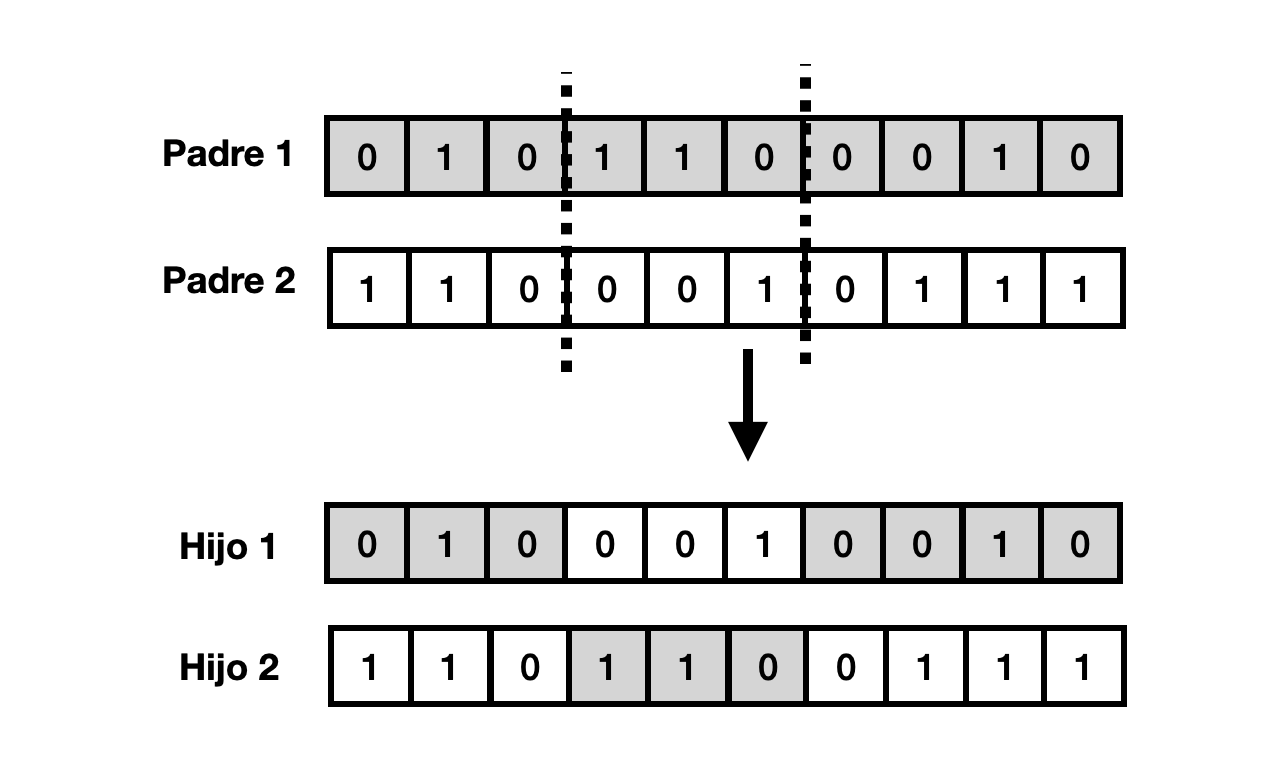
\includegraphics[width=0.9\textwidth]{images/crossOver.png}
  \caption{Ejemplo de crossover de dos puntos con dos cromosomas.}
  \label{fig:crossover}
\end{figure}


La Figura \ref{fig:crossover} muestra un ejemplo de cruzamiento para dos pares de padres con cromosomas representados como cadenas de bits. Los puntos de cruzamiento se encuentran después del tercer bit y después del sexto bit. Luego, se muestran los hijos o descendientes que se crean cruzando los cromosomas de los padres en los puntos de cruzamiento.

Para el primer par de padres, el descendiente resultante toma los primeros tres bits del primer padre, los tres bits siguientes del segundo padre y los últimos cuatro bits del primer padre. En cambio, para el segundo par de padres, el descendiente toma los primeros tres bits del segundo padre, los tres bits siguientes del primer padre y los últimos cuatro bits del primer padre.

En nuestro algoritmo, utilizamos un ratio de 0.30 para el cruzamiento, lo cual significa que en cada generación aproximadamente el 30 porciento de los individuos serán seleccionados para cruzarse y crear nuevos descendientes. Este valor fue obtenido a partir de evaluaciones experimentales que hemos realizado con 10 corridas del algoritmo.

El cruzamiento es una operación fundamental en los algoritmos genéticos, ya que permite combinar información genética de diferentes individuos y crear diversidad en la población, lo cual es esencial para la búsqueda de soluciones óptimas y la evolución del algoritmo.


\paragraph{Mutacion\pp{spell checker}}




La mutación es otro operador importante en los algoritmos genéticos. Consiste en introducir cambios aleatorios en los cromosomas de los individuos de la población para diversificar la búsqueda y evitar que el algoritmo quede atrapado en óptimos locales.

En el proceso de mutación, cada posición del estado de un individuo tiene una pequeña probabilidad de ser modificada. Esto significa que un bit en el estado puede cambiar de valor de manera aleatoria. Por ejemplo, si estamos representando los cromosomas como cadenas de bits, una mutación puede implicar cambiar un 0 por un 1 o viceversa.

Aunque la mutación es un proceso aleatorio, su probabilidad suele ser muy pequeña, generalmente en el rango de 0.01 a 0.05, para evitar que los cambios sean demasiado drásticos y permitir que los individuos mejor adaptados dominen la población. En nuestro algoritmo utilizamos 0.05.





El siguiente es el algoritmo genético que utilizamos para nuestra búsqueda
\\
\cacho{Algortimo? esta en preliminares, es standard para Genetico. Pongo los valores que utilizamos en cada parametros aca? Lo tengo en evaluacion.}
\\
%Pongo ejemplo de codigo???%
\begin{algorithm}[H]

\SetAlgoLined
\KwResult{Best solution}
Inicializar población inicial $P$ de cromosomas aleatorios\;

Evaluar la aptitud de cada cromosoma en $P$\;

\While{Criterio de terminación no se cumple}{ 
    Seleccionar cromosomas padres de $P$ para la reproducción\;
    Aplicar operador de cruce para generar descendencia\;
    Aplicar operador de mutación a la descendencia\;
    Evaluar la aptitud de los nuevos cromosomas\;
    % Reemplazar cromosomas menos aptos en $P$ por la descendencia\;
}
\caption{Algoritmo Genético}
\end{algorithm}
\pp{se queda muy corto este pseudocódigo, no explica casi nada.}
\pp{En este punto todavía no se sabe cuál es la función de fitness. No se
entiende que hace el algoritmo en el contexto de identificación de builders.}
\cacho{Explicar algortimo}

\subsection{Hill Climbing}
\label{alg:approachHC}
El algoritmo Hill Climbing, también conocido como búsqueda por ascenso de
colina\cite{Russell:2009}, es un algoritmo de búsqueda local que se utiliza para
optimizar una función de valoracion. El objetivo del algoritmo es encontrar la
solución óptima \pp{no es óptima} para un problema determinado.  Su enfoque se
basa en realizar movimientos ascendentes, es decir, buscar soluciones que
mejoren continuamente el valor objetivo o la función de evaluación \pp{o?}.
Este algoritmo es un algoritmo Greedy(Perezoso) explicado en la seccion de
preliminares, (\ref{sec:greedyPrev})\pp{no hay mucho que explicar en
preliminares sobre hill climbing, ya está todo acá por lo que veo}. Este selecciona un buen estado sucesor
para el momento actual, sin pensar en dónde ir a continuación \pp{no se entiende}. 
La idea principal detrás del algoritmo Hill Climbing es comenzar con una solución inicial y, en cada iteración, realizar un movimiento hacia una solución vecina que mejore el valor objetivo. Este proceso se repite hasta que no se pueda encontrar una solución vecina que mejore el valor actual. En ese punto, el algoritmo se detiene y devuelve la mejor solución encontrada hasta el momento.
Es importante destacar que el algoritmo Hill Climbing puede quedar atrapado en óptimos locales, es decir, puede converger hacia soluciones que son mejores en comparación con sus vecinos inmediatos, pero no son óptimas en el contexto global

La representación que hemos utilizado del problema fue igual a la que utilizamos para representar cromosomas en el Algoritmo genético explicado en la sección anterior. Esto quiere decir que utilizamos vectores de 0 y 1 para representar una posible solución. 

A continuación mostraremos un pseudocódigo del algoritmo \emph{Hill Climbing} que hemos implementado:
\pp{En este punto no se sabe cuál es la función de fitness, entonces no se
entiende que significa el algoritmo en el contexto de identificación de builders.}

\begin{algorithm}[H]
  \caption{Algoritmo de Hill Climbing}
  \label{algo:hill_climbing}
  \SetAlgoLined
  \KwResult{Solución óptima $curr$}
  $curr \gets c$\; 
  
  \While{existe un mejor candidato}{
    $S \gets$ GenerarSucesores($curr$)\;
    
    $best \gets$ SeleccionarMejorSucesor($S$)\;
    
    \If{$f(best) > f(curr)$}{
      $curr \gets best$\;
    }
  }
  \Return{$best$}\;
\end{algorithm}
\pp{Por qué devolver el return?}

Este algoritmo representa el esquema básico de Hill Climbing, comienza
calculando la funcion de valoración de todos los singletones ${c}$ de métodos
constructores.  El mejor de los singletones (mayor objectos puedo crear con ese
constructor) se establece como el candidato actual $curr$, y Hill Climbing
inicia un proceso de búsqueda típico e iterativo (Línea 1) \pp{Esto que se
explica acá no está en el algoritmo, hay una asignación nomás}.

En cada iteración (Línea 2 a 8), \emph{Hill Climbing} calcula $f(succ)$ para
cada succ $\in$ $GenerarSucesores(curr)$. El método que genera los sucesores nos
devuelve un conjunto de posibles soluciones que se crean a partir de sumarle un
método a la solución óptima corriente ($curr$). Es decir, los sucesores  $S$
generados con \emph{GenerarSucesores(curr)} de un candidato $curr$ son los
conjuntos {$curr\cup{mi}$}, para cada $mi$ $\in$ API (Línea 3) \pp{
Se podría poner el pseudocódigo de generar sucesores, y quizás poner un ejemplo
para que se entienda}.
Sea $best$ el sucesor con el valor de valoración más alto. Observe que $best$
tiene exactamente un método más que el mejor candidato de la iteración anterior,
$curr$ (Línea 4) \pp{hay que implementar con código el existe un mejor
candidato. Mirar el libro de AI.}.

Si $f(best) > f(curr)$, los métodos en $best$ se pueden utilizar para crear un
conjunto más grande de estructuras que los en $curr$ (Línea 5 a 7) \pp{f no está
definida}. Por lo tanto, \emph{Hill Climbing} asigna $best$ a $cur$r y continúa con la siguiente iteración. En cambio, si $f(best) <= f(curr)$, $curr$ ya genera el conjunto más grande de estructuras posible (no se puede agregar ningún método que aumente el número de estructuras generadas a partir de $curr$). En este punto, $curr$ se devuelve como el conjunto de constructores identificados. (Linea 9) 

% \cacho{
% En este algoritmo no se necesitan setear ningun parametros para guiar la busqueda a que sea mas efectiva}

Se puede observar que este algoritmo puede quedar atrapado en un máximo local y
no generar alguna combinación específica que podría ser aún mejor. Aquí se puede
ver que es un algoritmo greedy, ya que obtiene una solución rápida pero puede no
ser eficiente \pp{eficaz?} en encontrar la mejor solución global. 


\subsection{Clases de equivalencia}
\label{alg:approachCE}
 Las clases de equivalencia son una técnica utilizada para agrupar conjuntos de datos de entrada en categorías o clases que tienen un comportamiento similar o producen resultados equivalentes. Esta técnica es ampliamente utilizada en el diseño y la realización de pruebas de software.
 En términos generales, una clase de equivalencia representa  un conjunto de que se espera que produzcan resultados idénticos. La idea es que si un conjunto de la clase de equivalencia produce un resultado entonces todas las demás entradas de esa clase deberían producir el mismo resultado.
 Al trabajar con clases de equivalencia, se selecciona una entrada representativa, llamada caso de prueba, de cada clase para ser evaluada. En lugar de probar todas las posibles entradas, se eligen casos de prueba que representen cada clase de equivalencia para minimizar la cantidad total de pruebas necesarias.

 Bajo esta introducción, hemos desarrollado un tercer algoritmo donde agrupamos en clases de equivalencia aquellos subconjuntos de métodos que tengan el mismo valor de valoración con alguna de las funciones explicadas en \ref{sec:fitness}.


\begin{algorithm}[H]
  \caption{Algoritmo basado en Clases de Equivalencia}
  \label{algo:clases_equivalencia}
  \SetAlgoLined
  \KwResult{Conjunto de metodos builders $best$}
  $curr \gets c$\; 
  $equivalenceClasses \gets$ CrearClasesDeEquivalencia($curr$)\;
  
  \While{se ha creado una nueva clase de equivalencia}{
    $newCandidates \gets$ CandidatosPorClase($equivalenceClasses$)\;
    
    \ForEach{$candidate$ en $newCandidates$}{
      $successors \gets$ GenerarSucesores($candidate$)\;   
      
      \ForEach{$successor$ en $successors$}{
        $key \gets$ f($successor$)\;
        $equivalenceClasses[key]$.put($successor$)\;
      }
    }
        % $best \gets$ SeleccionarMejorCandidato($candidates$)\;
  }
  
  $result \gets$ obtenerMejor($best$)\;
  \Return{$result$}\;
\end{algorithm}

En este algoritmo, se comienza obteniendo los conjuntos singletons (Línea 1), que son los métodos constructores individuales de la misma manera que el algoritmo de \ref{algo:hill_climbing}. A partir de estos singletons, se selecciona el mejor candidato inicial $curr$, que servirá como punto de partida. Luego, se crean las clases de equivalencia basadas en la función de valoración y agrupando los candidatos que tienen el mismo valor de valoración. En el algortimo las clases de equivlencias estan guardadas en $equivalenceClasses$ (Línea 2).

A continuación, se itera (Línea 5 a 12) mientras se haya creado una nueva clase de equivalencia. En cada iteración, se generan nuevos candidatos por cada clase de equivalencia. Es decir, se selecciona un candidato de cada clase de equivalencia (el de menor métodos y menor parámetros) $CandidatosPorClase(equivalenceClasses)$ y se lo guarda en un cola ($newCandidates$) (Línea 5). A continuación, se generan los sucesores (línea 6) para cada candidato elegido, $GenerarSucesores(candidate)$, utilizando el mismo enfoque que en el algoritmo de \emph{Hill Climbing}. Estos se guardan en $successors$ Es decir, si tenemos $N$ clases de equivalencias vamos a tener $N$ candidatos a los cuales le vamos a calcular sus sucesores.  Luego, por cada uno de estos sucesores en  se le calcula su función de valoración y de acuerdo a esta se lo guarda en la clase de equivalencia representada por el valor de valoración.
El algoritmo itera hasta que no hayamos creado una nueva clase de equivalencia. Esto quiere decir que no hay cambios y hemos explorado todas las alternativas posibles. 
Luego vamos a obtener el mejor conjunto de métodos builders, accediendo a la clase de equivalencia con mayor key y obteniendo el representante de ese conjunto que tenga menor métodos y parámetros. Esto lo realiza el método $obtenerMejor(equivalenceClasses)$



\section{Función de Valoración}
\label{sec:fitness}


% En la búsqueda de soluciones óptimas mediante algoritmos genéticos u otros algoritmos de búsqueda, la función de valoración \cite{goldberg1989genetic} desempeña un papel fundamental. Su diseño adecuado es crucial, ya que determina la dirección y el éxito del proceso de búsqueda.
% La función de valoración evalúa la calidad de cada solución candidata y la compara con otras soluciones en la población. Proporciona una medida objetiva de la idoneidad de cada individuo en relación con los objetivos y restricciones del problema. La calidad se expresa generalmente mediante un valor numérico, donde valores más altos indican soluciones más deseables. Por ejemplo, si estamos resolviendo un problema de optimización en el que buscamos maximizar una función objetivo, la función de valoración puede asignar un valor más alto a las soluciones que se acercan más a la solución óptima. Por otro lado, si estamos resolviendo un problema de minimización, la función de valoración puede asignar un valor más alto a las soluciones que se alejan más de la solución óptima.
% Definir una buena función de valoración implica considerar cuidadosamente los requisitos y características del problema en cuestión. Puede implicar ponderar diferentes objetivos, como maximizar o minimizar ciertas variables, satisfacer restricciones específicas o lograr un equilibrio entre múltiples criterios. 

% Una función de valoración efectiva debe ser capaz de discriminar entre soluciones prometedoras y soluciones subóptimas. Debe proporcionar una evaluación objetiva y precisa, permitiendo la selección de soluciones de alta calidad y la eliminación de soluciones menos deseables.
% Además, la función de valoración debe ser adecuada para el dominio y el tipo de problema abordado. Puede requerir conocimiento especializado y experiencia en el campo para definir correctamente las métricas y ponderaciones apropiadas. 

% Es importante tener en cuenta que la función de valoración puede evolucionar y adaptarse a lo largo del proceso de búsqueda. A medida que el algoritmo de busqueda avanza y produce nuevas generaciones de soluciones, la función de valoración puede ser ajustada y refinada para enfocarse en las características más relevantes y deseadas.


% Por lo tanto, en los algoritmos de búsqueda la función de valoración desempeña un papel crucial para evaluar y comparar soluciones candidatas en función de criterios específicos del problema. Proporciona una medida cuantitativa de la calidad de las soluciones y guía el proceso de selección y toma de decisiones en cada etapa del algoritmo. El diseño adecuado de la función de valoración es esencial para obtener resultados óptimos y eficientes en la resolución de problemas.
% A continuación, explicaremos cada función de valoración implementada en nuestros algoritmos.


% En el caso de algoritmos greedy, la función de valoración juega un papel similar pero con un enfoque más local. En lugar de trabajar con una población de soluciones, los algoritmos greedy toman decisiones en cada paso basándose en una evaluación local de las opciones disponibles. La función de valoración en un algoritmo greedy se utiliza para seleccionar la mejor opción en cada iteración o paso del algoritmo, maximizando o minimizando la función de valoración según el objetivo del problema \cite{cormen2009introduction}.






\cacho{Tengo que agregar un cierre.}
